% /**
%  * @file manual.tex
%  * @author David Kvaček (xkvace00@stud.fit.vutbr.cz)
%  * @brief Project documentation from the ISA course.
%  * @date 2023-11-20
%  */

\documentclass[a4paper, 11pt]{article}

\usepackage[left=2cm, text={17cm, 25cm}, top=3cm]{geometry}
\usepackage[czech]{babel}
\usepackage[utf8]{inputenc}
\usepackage[IL2]{fontenc}
\usepackage{graphicx}
\usepackage{hyperref}

\begin{document}

\begin{titlepage}
    \begin{center}
        
\includegraphics[scale=0.125]{logo.png} \\
        \vspace{\stretch{0.382}}
        \LARGE{Dokumentace projektu z~předmětu ISA} \\
        \huge{\textbf{Monitorování DHCP komunikace}}
        \vspace{\stretch{0.618}}
    \end{center}

    \null \hfill \Large{David Kvaček} \\
    \Large{Brno, \today \hfill \href{mailto:xkvace00@stud.fit.vutbr.cz}{xkvace00@stud.fit.vutbr.cz}}
\end{titlepage}

\tableofcontents

\newpage

\section{Uvedení do problematiky}
Tato technická zpráva poskytuje podrobný pohled na návrh a~implementaci monitorovací aplikace DHCP komunikace.
Je zaměřena na analýzu síťové komunikace, konkrétně na protokol DHCP \cite{rfc2131}, a~přináší návrh efektivního nástroje pro sledování využívání adresového prostoru.
Dokumentace zahrnuje popis architektury aplikace (\ref{application-architecture}), postup implementace (\ref{implementation-process}) a~očekávané výstupy (\ref{output}).
Cílem je poskytnout užitečný nástroj pro správce sítí s~důrazem na optimalizaci a~bezpečnost síťové infrastruktury.

\subsection{Obecný popis aplikace}
Program \textbf{dhcp-stats} je uživatelská utilita umožňující získat statistiku o~vytížení síťového prefixu z~pohledu množství alokovaných IP adres.
Při zaplnění prefixu z~více jak 50\%, 75\%, 90\% a 95\%, nástroj informuje administrátora na standardní výstup a~zalogováním skrz \texttt{syslog} server \cite{syslog}.

Program po spuštění začne monitorovat DHCP provoz na zvoleném rozhraní, případně zpracuje \textit{pcap} soubor, a~generovat si statistiku vytížení síťového prefixu, který mu byl zadán v~příkazové řádce.
Prefixů může být více a~mohou se překrývat -- důvodem možného překryvu je zjištění, jak by vypadalo vytížení sítě, kdyby byl prefix větší.

\subsection{Protokol DHCP}
\textit{Dynamic Host Configuration Protocol} (DHCP) je síťový protokol používaný k~automatické konfiguraci síťových zařízení.
Jeho hlavním účelem je přidělovat IP adresy a~další síťové konfigurační informace zařízením v~síti.

DHCP funguje na klient-server modelu, kde DHCP server je zodpovědný za přidělování konfiguračních informací klientům v~síti.
Klienti, kteří připojí nové zařízení do sítě, komunikují s~DHCP serverem za účelem získání IP adresy, výchozí brány, DNS serveru a~dalších informací potřebných pro správnou komunikaci v~síti.

Proces začíná tím, že klient vysílá \texttt{DHCPDISCOVER} zprávu na síť, aby informoval o~své přítomnosti.
DHCP server odpovídá zprávou \texttt{DHCPOFFER}, ve které nabízí konfigurační informace, včetně přidělované IP adresy.
Klient poté posílá \texttt{DHCPREQUEST}, potvrzující přijetí nabízených informací.
Nakonec server odpovídá \texttt{DHCPACK}, potvrzující přidělení konfigurace klientovi \cite{dhcp}.

\begin{figure}[ht]
    \centering
    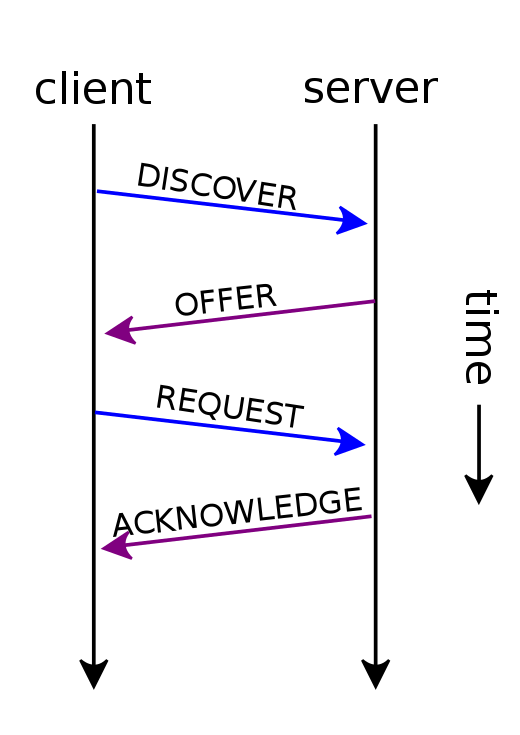
\includegraphics[scale=0.33]{dhcp-session.png}
    \caption{Ilustrace typické DHCP komunikace \cite{dhcp}}
    \label{dhcp-session}
\end{figure}

Protokol DHCP je klíčový pro správu síťových adres v~dynamických sítích, umožňuje snadnou a~efektivní konfiguraci nových zařízení a~minimalizuje potřebu manuálního zásahu do síťových nastavení.
Tato automatizace zvyšuje efektivitu správy sítě a~eliminuje riziko konfliktů IP adres, což je zásadní pro plynulý provoz moderních síťových infrastruktur.

Služby DHCP existují pro sítě s~internetovým protokolem verze 4 (IPv4) i~verze 6 (IPv6). Verze protokolu DHCP pro protokol IPv6 se běžně nazývá DHCPv6 \cite{dhcp}.

\newpage

\section{Návrh aplikace}
Výsledný uživatelský nástroj \textbf{dhcp-stats} má za cíl vylepšit optimalizaci a~správu síťové infrastruktury.
Aplikace slouží k~efektivnímu sledování a~analýze DHCP provozu, poskytující důležité informace o~využívání adresového prostoru.

\subsection{Architektura aplikace}
\label{application-architecture}
Utilita je implementována jako síťový sniffer, který zachytává a~analyzuje DHCP zprávy přenášené v~síti.
Pro dosažení tohoto cíle je použita specializovaná knihovna \texttt{libpcap} \cite{pcap} s~přidruženým hlavičkovým souborem \texttt{<pcap.h>}, která umožňuje odposlech a~dekódování DHCP komunikace.
Přijatá data jsou dále zpracována s~cílem získat informace o~přidělených IP adresách a~dalších relevantních parametrech.

\subsection{Princip fungování}
Jednou z~hlavních funkcí aplikace je shromažďování statistik o~vytíženosti zadaných IP prefixů.
To zahrnuje sledování toho, kolik IP adres z~konkrétního prefixu je aktuálně přiděleno zařízením v~síti.
Aplikace je schopna generovat přehledné a~jednoduché statistiky pro jednotlivé zadané prefixy, které umožní správcům sítě snadno identifikovat potenciální problémy s~přidělováním adres nebo neefektivním využíváním dostupného adresového prostoru.

\begin{figure}[ht]
    \centering
    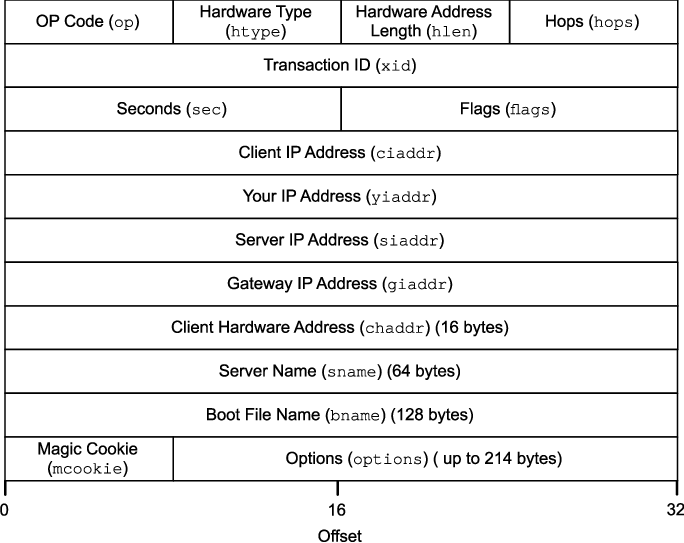
\includegraphics[scale=0.5]{dhcp-header.png}
    \caption{Formát hlavičky paketu DHCP protokolu \cite{dhcp-packet}}
    \label{dhcp-header}
\end{figure}

\newpage

\section{Popis implementace}
\label{implementation-process}
Implementace monitorování DHCP komunikace pro sledování vytíženosti zadaných IP prefixů vyžaduje integrovaný přístup k~síťové infrastruktuře a~systému, který dovoluje zachytávání a~analýzu DHCP paketů.
Celý program je navržen tak, aby umožnil sledování DHCP provozu na síti a~detekci vytížení definovaných IP prefixů.
Program je rozdělen do několika klíčových částí, které zajišťují efektivní a~bezproblémový chod.

\subsection{Implementační detaily}
Utilita \textbf{dhcp-stats} je napsána v~programovacím jazyce~C.
Pro práci se soubory \textit{pcap} a~monitorování síťových rozhraní je v~implementaci použita knihovna \texttt{libpcap} \cite{libpcap}.
Pro \textit{syslog} se používá standardní logovací rutina \texttt{syslog} \cite{syslog}.
Program \textbf{dhcp-stats} také předpokládá, že soubor \textit{pcap} nebo síťové rozhraní bude mít k~dispozici kompletní DHCP komunikaci, tj. jako kdyby byl nástroj spuštěn přímo na DHCP serveru.

\subsection{Struktura programu}
Veškerý zdrojový kód potřebný pro snadné spuštění utility se nachází ve třech souborech:
\begin{itemize}
    \item \texttt{dhcp-stats.c} -- zdrojový soubor v~programovacím jazyce~\texttt{C}.
    \item \texttt{dhcp-stats.h} -- hlavičkový soubor v~programovacím jazyce~\texttt{C}.
    \item \texttt{Makefile} -- funkční soubor pro překlad zdrojového souboru.
\end{itemize}

\subsubsection{Zdrojový soubor \texttt{dhcp-stats.c}}
Zdrojový soubor \texttt{dhcp-stats.c} obsahuje vlastní implementaci programu.
Pro přehlednost je kód uspořádán do několika jednoduchých funkcí, které zajišťují funkčnost a~chod celého nástroje.
Hlavní funkce programu \texttt{int main(int argc, char *argv[])} zpočátku provede kontrolu argumentů zadaných prostřednictvím příkazové řádky pomocí funkce \texttt{getopt()} \cite{getopt}.

Pokud tato funkce skončí úspěšně, přichází na řadu validace zadaných IP prefixů.
Tuto kontrolu má na svědomí jedna z~dalších funkcí \texttt{bool cidr\_validate(char *ip\_prefix)}.
Jak již z~prototypu funkce vyplývá, její návratová hodnota je \texttt{true}, nebo \texttt{false} a~na základě tohoto výsledku je zřejmé, zda-li zadaný IP prefix splňuje podmínku \textit{CIDR} notace \cite{cidr}.

V~tomto okamžiku je vše připraveno pro samotný běh programu.
Nejprve se alokuje odpovídající počet struktur sloužících k~uchovávání statistik jednotlivých prefixů podle jejich množství.
Inicializuje se standardní logovací rutina \texttt{syslog} \cite{syslog} a~okno \texttt{ncurses} \cite{ncurses} pro práci s~terminálem.

Následuje podstatná část programu, ve kterém se tok větví na dvě části.
Pokud byl zadán jako parametr programu \textit{pcap} soubor pomocí přepínače \texttt{-r}, nástroj zavolá odpovídající funkci, která zpracuje zadaný soubor -- \texttt{pcap\_t *pcap\_open\_offline(const char *, char *)}.
Druhou možností je funkce \texttt{pcap\_t *pcap\_open\_live(const char *, int, int, int, char *)}, která slouží k~zachytávání paketů v~reálném čase v~případě zadaného rozhraní přepínačem \texttt{-i}.

Pro analýzu a~detekci jednotlivých příchozích paketů v~rámci síťového provozu je použita tzv. \textit{callback} funkce \texttt{int pcap\_loop(pcap\_t *, int, pcap\_handler, u\_char *)}.
Jakmile je \textit{pcap} soubor zpracován nebo je ukončeno naslouchání na určitém rozhraní, program adekvátně ukončí všechny běžící procesy, zavře terminálové okno \texttt{ncurses} \cite{ncurses}, vypíše celkové statistiky na standardní výstup, uvolní veškerou alokovanou paměť, uzavře standardní logovací rutinu \texttt{syslog} \cite{syslog} a~skončí očekávaným návratovým kódem, případně, pokud nastala chyba, vypíše chybovou hlášku na standardní chybový výstup.

\subsubsection{Hlavičkový soubor \texttt{dhcp-stats.h}}
Hlavičkový soubor \texttt{dhcp-stats.h} obsahuje deklarace funkcí a~struktur pro implementaci uživatelské utility \textbf{dhcp-stats}, stejně jako všechny použité knihovny a~makra.
Soubor poskytuje rozhraní pro integraci s~hlavním programem, udržuje přehled o~využívaných funkcích a~použitých strukturách a~hraje klíčovou roli při oddělení rozhraní a~implementace, což usnadňuje čitelnost a~udržitelnost kódu.

Vzhledem k~nejednoznačnosti ve standardním hlavičkovém souboru \texttt{<netinet/udp.h>} \cite{udp} je použita vlastní struktura pro UDP hlavičku.
Tato struktura obsahuje standardní informace sloužící k~identifikaci zdrojového a~cílového portu, délky hlavičky a~kontrolní součet.
Deklarace struktury vypadá následovně:

\begin{verbatim}
    /**
      * @brief Structure for UDP header.
      * 
      */
    struct udp_hdr {
        u_int16_t uh_sport;
        u_int16_t uh_dport;
        u_int16_t uh_ulen;
        u_int16_t uh_sum;
    };
\end{verbatim}

Aby bylo možné dále pracovat přímo s~jednotlivými položkami daného DHCP paketu, je zapotřebí deklarovat strukturu DHCP hlavičky následovně:

\begin{verbatim}
    /**
     * @brief Structure for DHCP header.
     * 
     */
    struct dhcp_hdr {
        u_int8_t op;
        u_int8_t htype;
        u_int8_t hlen;
        u_int8_t hops;
        u_int32_t xid;
        u_int16_t secs;
        u_int16_t flags;
        struct in_addr ciaddr;
        struct in_addr yiaddr;
        struct in_addr siaddr;
        struct in_addr giaddr;
        u_int8_t chaddr[CHADDR];
        char sname[SNAME];
        char file[FILE];
        u_int32_t magic_cookie;
        u_int8_t options[OPTIONS];
    };
\end{verbatim}

Struktura pro uchovávání statistik jednotlivých prefixů je neméně důležitá.
Obsahuje nejen samotný IP prefix v~podobě textového řetězce pro jednoduché tisknutí statistik na standardní výstup, ale také maximální počet adres, které lze pro daný prefix alokovat, aktuální počet alokovaných adres a~samozřejmě procento, které udává aktuální vytížení IP prefixu v~podobě desetinného čísla.
Deklarace této struktury vypadá následujícím způsobem:

\begin{verbatim}
    /**
     * @brief Structure for DHCP statistics.
     * 
     */
    struct dhcp_stats {
        char *ip_prefix;
        u_int32_t max_hosts;
        u_int32_t allocated_addresses;
        double utilization;
    };
\end{verbatim}

\subsubsection{Funkční soubor \texttt{Makefile}}
\texttt{Makefile} je konfigurační soubor pro sestavování programu.
Cíle v~tomto souboru popisují, jak překladač a~linker mají sestavit projekt.
Základní cíle obvykle zahrnují kompilaci zdrojových souborů, vytvoření spustitelného souboru a~čištění dočasných souborů.
Proměnné jsou použity pro definici překladače, volby překladu a~dalších parametrů.

\texttt{Makefile} také obsahuje pravidla pro závislosti mezi soubory, což zajišťuje efektivní sestavení pouze změněných částí.
Jednoduchý, ale mocný nástroj, který zjednodušuje proces sestavování a~udržuje projekt dobře organizovaný.

Tento specifický \texttt{Makefile} slouží k~sestavení programu \textbf{dhcp-stats} pomocí veřejně známého příkazu \texttt{make}.
Kompilace se provádí pomocí překladače \texttt{gcc} \cite{gcc} s~nastavenými standardy \texttt{std=gnu17}, přičemž všechna varování jsou striktně brána jako chyby (\texttt{-Wall -Werror -Wextra -pedantic}).
Program využívá knihoven \texttt{-lpcap}, \texttt{-lm} a~\texttt{-lncurses}.
Cílovým souborem je \texttt{dhcp-stats}, který je generován z~\texttt{dhcp-stats.c}.

\texttt{Makefile} obsahuje také cíle pro vytvoření archivu zdrojových souborů a~dokumentace ve formátu tar \texttt{make tar}.
Pro čištění souborů kompilace a~archivu ve formátu tar je k~dispozici cíl \texttt{make clean}.

\subsection{Zajímavé pasáže implementace}
Projekt je členěn do několika souborů a~jednotlivé soubory do několika jednoduchých a~přehledných funkcí.
I~přesto lze představit dvě zajímavé funkce celého programu.

\subsubsection{Funkce \texttt{within\_range()}}
Funkce \texttt{bool within\_range(struct in\_addr, char *)} slouží k~ověření, zda zadaná IP adresa patří do daného rozsahu definovaného IP prefixem.
Funkce přijímá strukturu \texttt{struct in\_addr} reprezentující adresu a~řetězec \texttt{char *}, obsahující IP adresu a~masku ve formátu \textit{adresa/maska}.

Funkce nejprve parsováním získává IP adresu a~masku z~prefixu.
Poté převádí IP adresu na síťovou adresu.
Následně vypočítá adresu sítě a~broadcastovou adresu pomocí masky.
Dalším krokem je porovnání zadané adresy s~vypočítaným rozsahem a~vrácení \texttt{true}, pokud adresa patří do rozsahu, v~opačném případě \texttt{false}.

V~případě, že maska je minimální (\texttt{/0}), funkce kontroluje, zda adresa není adresa sítě nebo broadcastová adresa.
Pro masku maximální (\texttt{/32}) vrací vždy \texttt{false}.
Pro ostatní masky porovnává, zda zadaná adresa leží mezi vypočítanou adresou sítě a~broadcastovou adresou.

\subsubsection{Funkce \texttt{packet\_handler()}}
Funkce \texttt{void packet\_handler(u\_char *, const struct pcap\_pkthdr *, const u\_char *)} slouží k~analýze paketů zachycených pomocí knihovny \texttt{libpcap} \cite{pcap}.
Nejprve zjišťuje, zda se jedná o~paket s~protokolem IP a~UDP \cite{udp}, přičemž následně ověřuje, zda je port DHCP serveru 67 a~cílový port DHCP klienta 68 a~také zda paket obsahuje validní položku \texttt{magic\_cookie} \cite{rfc2131}.

Pokud jsou splněny všechny podmínky, funkce kontroluje, zda není nově zjištěná adresa již přidělená.
Pokud ne, přidá ji do seznamu přidělených adres a~aktualizuje statistiky pro odpovídající IP prefix.
V~případě překročení určitých procentuálních limitů (50\%, 75\%, 90\% a~95\%) využití přidělených adres v~rámci daného prefixu, funkce generuje systémový log pomocí standardní logovací rutiny \texttt{syslog} \cite{syslog} a~vypisuje upozornění na standardní výstup.

Nakonec funkce aktualizuje a~zobrazuje tabulku s~aktuálními statistikami využití IP prefixů, což poskytuje přehled o~maximálním počtu alokovatelných adres, počtu aktuálně přidělených adres a~procentuálním využití jednotlivých prefixů.

Tato funkce je volána jako tzv. \textit{callback} při každém zachyceném paketu během monitorování síťového provozu a~slouží ke sledování a~zaznamenávání statistik ohledně přidělovaných IP adresách DHCP serverem a~jedná se v~podstatě o~hlavní jádro celého programu.

\subsection{Funkční omezení}
\begin{itemize}
    \item Nástroj \textbf{dhcp-stats} nepodporuje adresy IPv6 a~komunikaci DHCPv6.
    \item Zprávy \texttt{DHCPRELEASE}, \texttt{DHCPDECLINE} a~aktualizace obsazenosti síťových prefixů na základě vypršení \textit{lease-time} nejsou podporovány.
    \item Utilita \textbf{dhcp-stats} také předpokládá DHCP komunikaci na standardních portech 67 a~68.
\end{itemize}

\newpage

\section{Návod na použití}
Minimální konfigurace pro úspěšný překlad a~spuštění programu nezbytně vyžaduje následující prvky:
\begin{itemize}
    \item GNU kompilátor (\texttt{gcc}) ve verzi podporující standard \texttt{gnu17} \cite{gcc}.
    \item Balíček \texttt{libpcap} pro zachytávání paketů (\texttt{<pcap.h>}) \cite{libpcap}.
    \item Knihovna \texttt{-lm} pro matematické operace (\texttt{<math.h>}) \cite{math}.
    \item Knihovna \texttt{-lncurses} pro práci s terminálem (\texttt{<ncurses.h>}) \cite{ncurses}.
\end{itemize}

\subsection{Použití}
\begin{verbatim}
    $ ./dhcp-stats [-h] [-r <filename>] [-i <interface-name>] <ip-prefix> [ ... ]
\end{verbatim}

\begin{enumerate}
    \item[] \texttt{-h} -- zobrazení nápovědy k~použití na standardní výstup a~ukončení.
    \item[] \texttt{-r <filename>} -- statistika bude vytvořena z~\textit{pcap} souboru.
    \item[] \texttt{-i <interface-name>} -- rozhraní, na kterém může program naslouchat.
    \item[] \texttt{<ip-prefix>} -- rozsah sítě, pro které se bude generovat statistika.
\end{enumerate}

\subsection{Status ukončení}
Program \textbf{dhcp-stats} skončí s~návratovou hodnotou 0~v~případě úspěchu a~s~návratovou hodnotou $>$0~v~případě chyby.

\subsection{Příklad spuštění}
Zpracování DHCP komunikace z~\textit{pcap} souboru \texttt{homenetwork.pcap} pro síťové prefixy \texttt{192.168.1.0/24}, \texttt{192.168.0.0/22} a~\texttt{172.16.32.0/24}:

\begin{verbatim}
    $ ./dhcp-stats -r homenetwork.pcap 192.168.1.0/24 192.168.0.0/22 172.16.32.0/24
\end{verbatim}

Monitorování DHCP komunikace na rozhraní \texttt{eth0} pro síťové prefixy \texttt{192.168.1.0/24}, \\\texttt{192.168.0.0/22} a~\texttt{172.16.32.0/24}:

\begin{verbatim}
    $ ./dhcp-stats -i eth0 192.168.1.0/24 192.168.0.0/22 172.16.32.0/24
\end{verbatim}

\subsection{Výstup}
\label{output}
\begin{verbatim}
    $ ./dhcp-stats -i eth0 192.168.1.0/24 192.168.0.0/22 172.16.32.0/24
    IP-Prefix Max-hosts Allocated addresses Utilization
    192.168.0.0/22 1022 123 12.04%
    192.168.1.0/24 254 123 48.43%
    172.16.32.0/24 254 15 5.9%
\end{verbatim}

\subsection{Logování}
V~případě, že počet alokovaných adres v~prefixu překročí 50\%, 75\%, 90\% a~95\%, program tuto informaci zaloguje skrz standardní \texttt{syslog} \cite{syslog} mechanismus do logu následovně:

\begin{verbatim}
    prefix x.x.x.x/y exceeded 50% of allocations
    prefix x.x.x.x/y exceeded 75% of allocations
    prefix x.x.x.x/y exceeded 90% of allocations
    prefix x.x.x.x/y exceeded 95% of allocations
\end{verbatim}

\newpage

\section{Seznam odevzdaných souborů}
\begin{itemize}
    \item \texttt{dhcp-stats.1} -- soubor ve formátu a~syntaxi manuálové stránky \cite{manpage}.
    \item \texttt{dhcp-stats.c} -- zdrojový soubor v~programovacím jazyce~\texttt{C}.
    \item \texttt{dhcp-stats.h} -- hlavičkový soubor v~programovacím jazyce~\texttt{C}.
    \item \texttt{Makefile} -- funkční soubor pro překlad zdrojového souboru.
    \item \texttt{manual.pdf} -- soubor obsahující dokumentaci projektu ve formátu \texttt{PDF}.
    \item \texttt{README} -- soubor ve formátu a~syntaxi jazyka \texttt{Markdown} \cite{markdown}.
\end{itemize}

\newpage

\section{Literatura}
\bibliographystyle{czechiso}
\renewcommand{\refname}{}
\bibliography{manual}

\end{document}
